\section*{Assignment 2: Time Domain Transmission Lines}

During this assignment, the setup in figure \ref{fig:ass2_setup1} was used. It consisted of a pulse generator which sends a square pulse to a DUT (device under test) via a coax cable (with $Z_0 = 50 \Omega$), a sampling unit, which samples the electric field in the coax cable, and an oscilloscope, which measures the sampled electric field strength.\\

\begin{figure}[H]
	\centering
	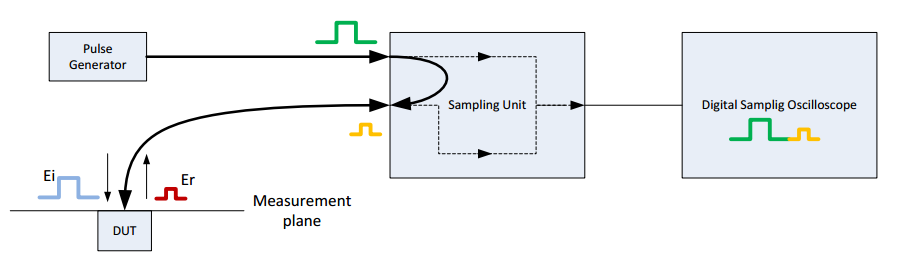
\includegraphics[width=\textwidth]{ass2_setup1.png}
	\caption{Experimental set-up for Assignment 2}
	\label{fig:ass2_setup1}
\end{figure}

\subsection*{Time Domain Reflectometry}

In this part, the reflection of an incident square pulse was investigated. As the oscilloscope measured the total electric field in the coax cable, it also registered the reflection of the pulse, from which the reflection coefficient was be derived. Three loads were used: a short circuit, a matched load, and an unknown load. The three measurements were plotted together an shown below in figure \ref{fig:results2}.

\begin{figure}[H]
	\centering
	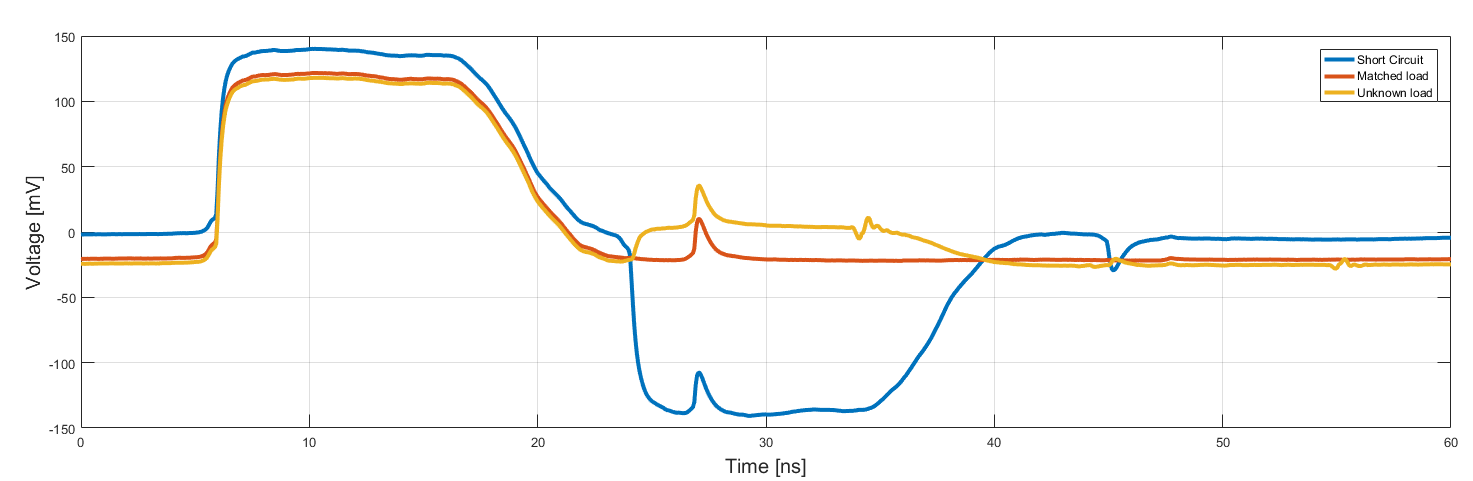
\includegraphics[width=\textwidth]{results2.png}
	\caption{Experimental set-up for Assignment 2}
	\label{fig:results2}
\end{figure}

From transmission line theory \cite{textbook}, we know that the reflection coefficient can be written as shown below in equation \ref{eq:reflect_co}.

\begin{equation}
\Gamma = \frac{Z_L - Z_0}{Z_L + Z_0}
\label{eq:reflect_co}
\end{equation}

From this, equation \ref{eq:reflect_amp} follows:

\begin{equation}
V^r = \Gamma \cdot V^i
\label{eq:reflect_amp}
\end{equation}

Using the equations, we can evaluate the two known loads, and determine the unknown load as well/
\begin{enumerate}
	\item Short Circuit: With a short circuit, $Z_L$ = 0, which gives a reflection co\"eficient of $\Gamma = -1$.  From figure \ref{fig:results2} we see that the peak of $V^i$ is 140mV, and that $V^r$ is -140mV, which is also to be expected.

	\item Matched Load: For the matched load, we see that $Z_L$ = $Z_0$, which gives a reflection co\"eficient of $\Gamma = 0$. Figure \ref{fig:results2} also shows that the matched load has no reflection, which agrees with the above reflection co\"eficient.
	
	\item Unknown Load: Figure \ref{fig:results2} gives $V^i$ as 140mV, and $V^r$ as 28mV. This gives a reflection co\"eficient of approximately 0.2. Know that $Z_0 = 50 \ \Omega$ from the experiment, we calculate that the unknown load is $Z_L = 75 \ \Omega$.
\end{enumerate}

Is the cases above, only the real parts of the reflection co\"eficient and load impedance are calculated, as only the amplitude of the signals were looked at. By investigating the phase shift of the signals, we could also calculated the imaginary parts. Looking at the results in figure \ref{fig:results2}, we can see very little phase shift in the reflected signals, which is also to be expected, as imaginary loads are typically dominated by the cable length and construction, as discussed in the next section.

\subsection*{Propagation speed and relative permittivity}

The experimental set-up was adjusted so that the delay in a coaxial cable can be measured. The results of the measurements can be see below in figure \ref{fig:results3}.

\begin{figure}[H]
	\centering
	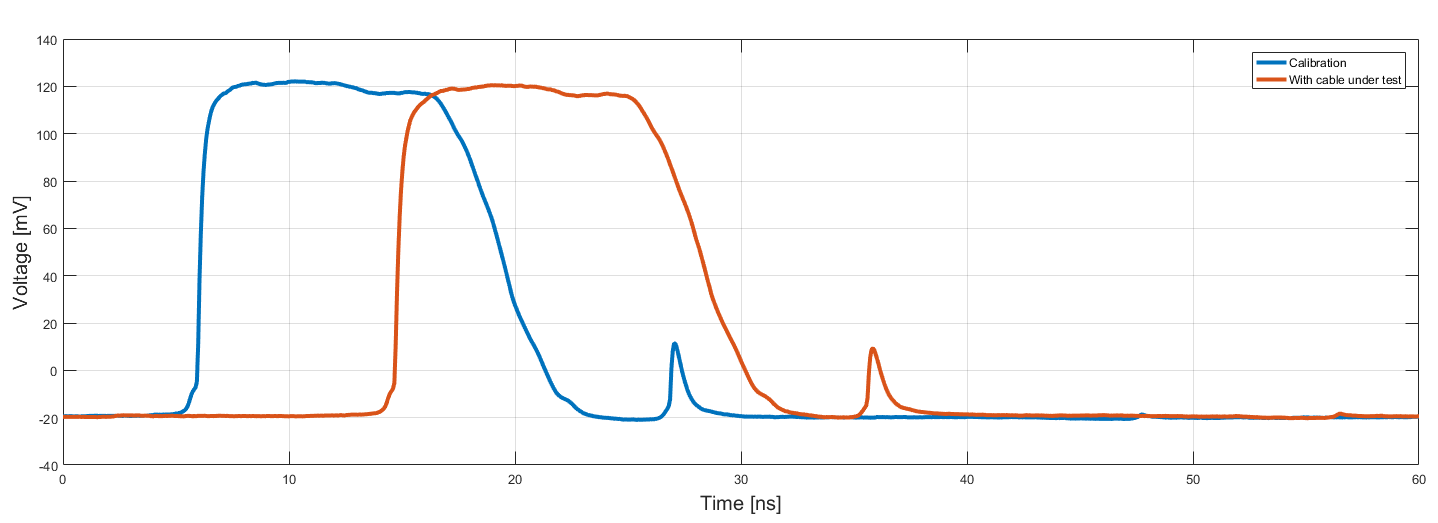
\includegraphics[width=\textwidth]{results3.png}
	\caption{Experimental set-up for Assignment 2}
	\label{fig:results3}
\end{figure}

For the results, we see the expected phase shift due to the varying cable lengths. The cable construction forms a capacitance between the outer shield and core, which is dependant of the diameter, the cable length, and the di-electric of the insulator. We can calculate the difference in the relative permittivity of the di-electric insulators between the two cables.

Looking at the graph, we can see that the delay between the two rising edges is approximately \SI{8.8}{\nano\second}. Given that the cable was \SI{2}{\meter} long, we calculate the propagation speed in the cable to be $2.2 \cdot{10^8}$ \SI{}{\meter\per\second}. From transmission line theory \cite{textbook} we get equation \ref{eq:prop_speed} below, where $\mu_r$ is the relative permeability, and $\epsilon_r$ is the relative permittivity.

\begin{equation}
c = (\mu\epsilon)^{-1} = c_0(\mu_r\epsilon_r)^{-1}
\label{eq:prop_speed}
\end{equation}

Assuming the relative permeability to be 1, we can compare the speeds of the EM waves in the two cables, and determine the relative permittivity of the cable dielectric, as shown below in equation \ref{rel_perm}.

\begin{equation}
\sqrt{\epsilon_r\mu_r} = \frac{c_0}{c} \Leftrightarrow
\epsilon_r = \left(\frac{c_0}{c}\right)^2 = \left(\frac{3 \cdot 10^8 \text{ m/s}}{2.2 \cdot 10^8 \text{ m/s}}\right)^2 \approx 1.86
\label{rel_perm}
\end{equation}

